
%  Adaptive Multigrid FSP for the RDME — Talk Slides (ver 2)
%  Aditya Dendukuri

\documentclass[10pt,aspectratio=169]{beamer}

\usetheme{Boadilla}
\usecolortheme{seahorse}
\setbeamertemplate{navigation symbols}{}
\setbeamerfont{frametitle}{size=\normalsize,series=\bfseries}
\setbeamerfont{title}{size=\large,series=\bfseries}
\setbeamertemplate{bibliography item}[text]

\usepackage{pgfpages}
\pgfpagesuselayout{resize to}[physical paper width=33.87cm,physical paper height=19.05cm]

\usepackage{amsmath,amssymb,bm,mathtools}
\usepackage{tikz}
\usetikzlibrary{arrows.meta,positioning,patterns,decorations.pathreplacing,calc}
\usepackage{graphicx}
\usepackage{booktabs}
\usepackage{xcolor}
\usepackage[numbers,sort&compress]{natbib}
\usepackage{pifont}
\usepackage{algorithm}
\usepackage{algorithmic}
\renewcommand{\algorithmicrequire}{\textbf{Input:}}
\renewcommand{\algorithmicensure}{\textbf{Output:}}

\graphicspath{{figures/}}

\newcommand{\bx}{\mathbf{x}}
\newcommand{\Znn}{\mathbb{Z}_{\geq 0}}
\newcommand{\E}{\mathbb{E}}
\newcommand{\TV}{\operatorname{TV}}
\newcommand{\Bin}{\operatorname{Bin}}
\newcommand{\calR}{\mathcal{R}}
\newcommand{\calP}{\mathcal{P}}
\newcommand{\norm}[1]{\left\|#1\right\|}
\newcommand{\citeref}[1]{{\scriptsize\textcolor{gray}{[#1]}}}

\definecolor{fastblue}{RGB}{31,119,180}
\definecolor{slowred}{RGB}{214,39,40}
\definecolor{coarsegreen}{RGB}{44,160,44}
\definecolor{finecolor}{RGB}{214,39,40}
\definecolor{coarsecolor}{RGB}{31,119,180}
\definecolor{intercolor}{RGB}{255,140,0}
\definecolor{myblue}{RGB}{31,119,180}
\definecolor{mygray}{RGB}{80,80,80}

\title[Adaptive Multigrid FSP]{%
  Adaptive Multigrid Finite State Projection\\
  for the Reaction-Diffusion Master Equation}
\author{Aditya Dendukuri}
\institute[UCSB]{University of California, Santa Barbara}
\date{}


\begin{document}

\begin{frame}
  \titlepage
\end{frame}


% ================================================================
%  1.  The problem: RDME state space is huge
% ================================================================

\begin{frame}{The RDME: reactions and diffusion across a spatial grid}

  \begin{columns}[T]
    \begin{column}{0.50\textwidth}
      \textbf{Model.}
      Divide a 1-D domain into $K$ voxels.
      Each voxel $k$ holds molecule counts $\mathbf{n}_k \in \mathbb{Z}_{\geq 0}^S$.

      \medskip
      Two types of events:
      \begin{itemize}\setlength\itemsep{0.4em}
        \item \textcolor{slowred}{\textbf{Reactions}} inside voxel $k$:
              rate $\alpha_r(\mathbf{n}_k)$, change $\mathbf{n}_k$.
        \item \textcolor{fastblue}{\textbf{Diffusion}} between neighbors:
              rate $d = D/h^2$, moves one molecule $k \leftrightarrow k{+}1$.
      \end{itemize}

      \medskip
      The joint probability $p(\mathbf{n}_1,\ldots,\mathbf{n}_K,t)$
      satisfies $\dot p = A p$ \textbf{(RDME)}.

      \medskip
      \begin{alertblock}{The computational bottleneck}
        The state space has $\sim n_{\max}^{SK}$ reachable states —
        \textbf{exponential in $K$}.
        Even $K{=}8$, $S{=}1$ is intractable with a naive FSP.
      \end{alertblock}
    \end{column}
    \begin{column}{0.46\textwidth}
      \begin{center}
      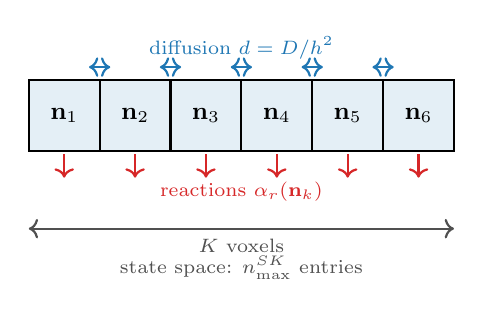
\begin{tikzpicture}[scale=0.90, every node/.style={font=\small}]
        % Voxels
        \foreach \k in {1,2,3,4,5,6} {
          \draw[thick,fill=myblue!12] (\k-1,0) rectangle (\k,1.0);
          \node at (\k-0.5, 0.50) {$\mathbf{n}_\k$};
        }
        % Diffusion arrows
        \foreach \k in {1,2,3,4,5} {
          \draw[<->,fastblue,thick] (\k-0.15,1.18) -- (\k+0.15,1.18);
        }
        \node[fastblue, font=\scriptsize] at (3, 1.45) {diffusion $d = D/h^2$};
        % Reaction arrows
        \foreach \k in {1,2,3,4,5,6} {
          \draw[->,slowred,thick] (\k-0.5,-0.05) -- (\k-0.5,-0.38);
        }
        \node[slowred, font=\scriptsize] at (3, -0.58) {reactions $\alpha_r(\mathbf{n}_k)$};

        % State space label
        \draw[<->,thick,mygray] (0,-1.1) -- (6,-1.1)
          node[midway,below,font=\scriptsize]{$K$ voxels};
        \node[mygray,font=\scriptsize] at (3,-1.65)
          {state space: $n_{\max}^{SK}$ entries};
      \end{tikzpicture}
      \end{center}
    \end{column}
  \end{columns}

\end{frame}


% ================================================================
%  1b.  The generator: block-tridiagonal structure
% ================================================================

\begin{frame}{The probability ODE $\dot{p} = Ap$ has block-tridiagonal structure \textnormal{\small(schematic, $K{=}4$, $S{=}1$)}}

\vspace{-0.2cm}
\begin{center}
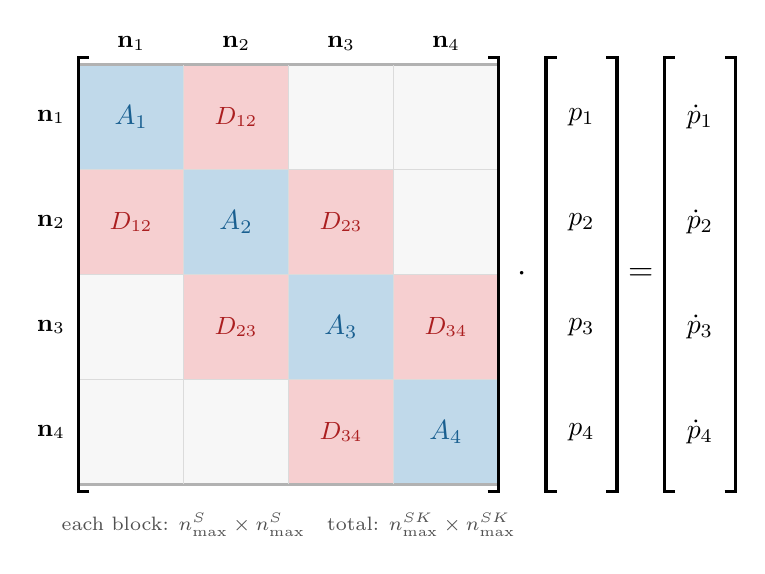
\begin{tikzpicture}[scale=0.86]
  \def\bs{1.55}   % block size
  \def\bw{0.16}   % bracket arm width
  \def\bp{0.10}   % bracket padding

  \fill[gray!6] (0,0) rectangle (4*\bs,4*\bs);

  \foreach \k in {0,1,2,3}
    \fill[myblue!28] (\k*\bs,{(3-\k)*\bs}) rectangle ({(\k+1)*\bs},{(4-\k)*\bs});

  \foreach \k in {0,1,2} {
    \fill[slowred!22] ({(\k+1)*\bs},{(3-\k)*\bs})
                   rectangle ({(\k+2)*\bs},{(4-\k)*\bs});
    \fill[slowred!22] ({\k*\bs},{(2-\k)*\bs})
                   rectangle ({(\k+1)*\bs},{(3-\k)*\bs});
  }

  \draw[black!30,thick] (0,0) rectangle (4*\bs,4*\bs);
  \foreach \k in {1,2,3} {
    \draw[black!14,thin] (\k*\bs,0) -- (\k*\bs,4*\bs);
    \draw[black!14,thin] (0,\k*\bs) -- (4*\bs,\k*\bs);
  }

  \foreach \k/\l in {0/1,1/2,2/3,3/4}
    \node[font=\normalsize, myblue!80!black]
      at ({(\k+0.5)*\bs},{(3.5-\k)*\bs}) {$A_\l$};
  \node[font=\small,slowred!80!black] at (1.5*\bs,3.5*\bs) {$D_{12}$};
  \node[font=\small,slowred!80!black] at (0.5*\bs,2.5*\bs) {$D_{12}$};
  \node[font=\small,slowred!80!black] at (2.5*\bs,2.5*\bs) {$D_{23}$};
  \node[font=\small,slowred!80!black] at (1.5*\bs,1.5*\bs) {$D_{23}$};
  \node[font=\small,slowred!80!black] at (3.5*\bs,1.5*\bs) {$D_{34}$};
  \node[font=\small,slowred!80!black] at (2.5*\bs,0.5*\bs) {$D_{34}$};

  % ── Column / row headers (voxel state) ──────────────────────────
  \foreach \k/\l in {0/$\mathbf{n}_1$,1/$\mathbf{n}_2$,2/$\mathbf{n}_3$,3/$\mathbf{n}_4$} {
    \node[above,font=\small] at ({(\k+0.5)*\bs}, 4*\bs+0.06) {\l};
    \node[left, font=\small] at (-0.06, {(3.5-\k)*\bs}) {\l};
  }

  % ── Matrix brackets ─────────────────────────────────────────────
  \draw[very thick]
    (\bw,-\bp) -- (0,-\bp) -- (0,4*\bs+\bp) -- (\bw,4*\bs+\bp);
  \draw[very thick]
    (4*\bs-\bw,-\bp) -- (4*\bs,-\bp) -- (4*\bs,4*\bs+\bp) -- (4*\bs-\bw,4*\bs+\bp);

  % ── × p ─────────────────────────────────────────────────────────
  \def\vgap{0.70}   % gap between matrix and vector
  \def\vw{1.05}     % vector column width
  \pgfmathsetmacro{\vx}{4*\bs + \vgap}

  \node[font=\large] at ({4*\bs + \vgap/2}, {2*\bs}) {$\cdot$};

  \draw[very thick]
    (\vx+\bw,-\bp) -- (\vx,-\bp) -- (\vx,4*\bs+\bp) -- (\vx+\bw,4*\bs+\bp);
  \draw[very thick]
    (\vx+\vw-\bw,-\bp) -- (\vx+\vw,-\bp) -- (\vx+\vw,4*\bs+\bp)
    -- (\vx+\vw-\bw,4*\bs+\bp);

  \foreach \k/\l in {0/$p_1$,1/$p_2$,2/$p_3$,3/$p_4$}
    \node[font=\normalsize] at (\vx+\vw/2, {(3.5-\k)*\bs}) {\l};

  % ── = ───────────────────────────────────────────────────────────
  \pgfmathsetmacro{\eqx}{\vx + \vw + \vgap/2}
  \node[font=\large] at (\eqx, {2*\bs}) {$=$};

  % ── dp/dt vector ────────────────────────────────────────────────
  \pgfmathsetmacro{\rx}{\vx + \vw + \vgap}

  \draw[very thick]
    (\rx+\bw,-\bp) -- (\rx,-\bp) -- (\rx,4*\bs+\bp) -- (\rx+\bw,4*\bs+\bp);
  \draw[very thick]
    (\rx+\vw-\bw,-\bp) -- (\rx+\vw,-\bp) -- (\rx+\vw,4*\bs+\bp)
    -- (\rx+\vw-\bw,4*\bs+\bp);

  \foreach \k/\l in {0/$\dot p_1$,1/$\dot p_2$,2/$\dot p_3$,3/$\dot p_4$}
    \node[font=\normalsize] at (\rx+\vw/2, {(3.5-\k)*\bs}) {\l};

  % ── size annotation ─────────────────────────────────────────────
  \node[mygray,font=\scriptsize,below] at (2*\bs,-\bp-0.18)
    {each block: $n_{\max}^S \times n_{\max}^S$\quad total: $n_{\max}^{SK} \times n_{\max}^{SK}$};

\end{tikzpicture}
\end{center}

\vspace{0.3em}
{\small
  \textcolor{myblue!80!black}{$A_k$}: reactions inside voxel $k$
  \hspace{1.5em}
  \textcolor{slowred!80!black}{$D_{k,k+1}$}: diffusion between neighboring voxels
  \hspace{1.5em}
  $p_k$: probability sub-vector for voxel $k$'s state
}

\end{frame}



\begin{frame}{The Binomial is the exact diffusion equilibrium}

  \begin{columns}[T]
    \begin{column}{0.50\textwidth}
      \textbf{Fix total molecules} $\bar n = n_1 + n_2$ across two adjacent voxels.

      \smallskip
      Diffusion moves one molecule at a time, at rate $d$ per molecule:

      \begin{center}
      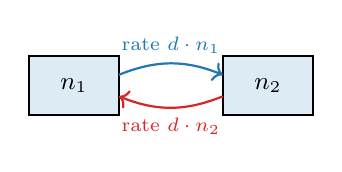
\begin{tikzpicture}[every node/.style={font=\small}, scale=0.88]
        \draw[thick,fill=coarsecolor!15] (0,0) rectangle (1.3,0.85);
        \draw[thick,fill=coarsecolor!15] (2.8,0) rectangle (4.1,0.85);
        \node at (0.65, 0.42) {$n_1$};
        \node at (3.45, 0.42) {$n_2$};
        \draw[->,fastblue,thick,bend left=22] (1.3,0.58)
          to node[above,font=\scriptsize]{rate $d\cdot n_1$} (2.8,0.58);
        \draw[->,slowred,thick,bend left=22]  (2.8,0.27)
          to node[below,font=\scriptsize]{rate $d\cdot n_2$} (1.3,0.27);
      \end{tikzpicture}
      \end{center}

      Each molecule hops independently, so at equilibrium it is equally
      likely to be in either voxel. For $\bar n$ total:
      \[
        \boxed{P(n_1 \mid \bar n) = \Bin\!\bigl(\bar n,\,\tfrac{1}{2}\bigr)}
        \quad \text{(exact, any } d > 0\text{)}
      \]
      When the distribution is near this equilibrium
      (checked at runtime via $\alpha_j$),
      \textbf{$\bar n$ alone describes the two-voxel state}.
    \end{column}
    \begin{column}{0.46\textwidth}
      \begin{center}
      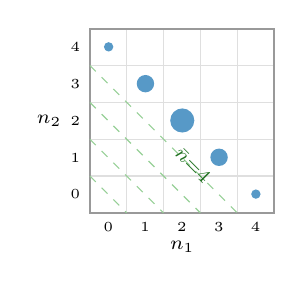
\begin{tikzpicture}[scale=0.85]
        \def\cs{0.55}
        \draw[gray!25](0,0) grid[step=\cs] (5*\cs,5*\cs);
        \draw[black!40,thick](0,0) rectangle (5*\cs,5*\cs);
        % Constant-total diagonals
        \foreach \t in {1,2,3,4} {
          \draw[coarsegreen!50,dashed,thin]
            ({max(0,\t-4)*\cs},{min(\t,4)*\cs}) -- ({min(\t,4)*\cs},{max(0,\t-4)*\cs});
        }
        % Binomial masses on the \bar n = 4 diagonal
        \fill[coarsecolor!75](0.28,2.48) circle (0.07cm);
        \fill[coarsecolor!75](0.83,1.93) circle (0.13cm);
        \fill[coarsecolor!75](1.38,1.38) circle (0.18cm);
        \fill[coarsecolor!75](1.93,0.83) circle (0.13cm);
        \fill[coarsecolor!75](2.48,0.28) circle (0.07cm);
        % Axis labels
        \foreach \n in {0,1,2,3,4}
          \node[below,font=\tiny] at ({(\n+0.5)*\cs},0) {\n};
        \foreach \n in {0,1,2,3,4}
          \node[left,font=\tiny]  at (0,{(\n+0.5)*\cs}) {\n};
        \node[below,font=\scriptsize] at (1.38,-0.28) {$n_1$};
        \node[left, font=\scriptsize] at (-0.28,1.38) {$n_2$};
        \node[coarsegreen!70!black,font=\scriptsize,rotate=-45] at (2.8*\cs,1.3*\cs) {$\bar n{=}4$};
      \end{tikzpicture}

      \vspace{0.4em}
      {\footnotesize
        Probability is spread along each constant-total diagonal
        as $\Bin(\bar n,\tfrac12)$ (dot size $\propto$ mass).\\[0.3em]
        \textbf{The two-voxel state is captured by $\bar n$ alone.}
      }
      \end{center}
    \end{column}
  \end{columns}

\end{frame}



\begin{frame}{Merging two adjacent voxels into their total}

  \begin{columns}[T]
    \begin{column}{0.50\textwidth}
      \textbf{Compress ($\calR$) — exact:}
      \[ p^c(\bar n) = \!\!\sum_{n_1 + n_2 = \bar n}\!\! p(n_1, n_2). \]

      \textbf{Reconstruct ($\calP$) — approximate:}
      \[ p(n_1, n_2) \approx p^c(\bar n)\cdot\Bin(\bar n,\tfrac{1}{2}). \]

      \begin{block}{State-space reduction}
        Per block: $n_{\max}^{2S} \to n_{\max}^{S}$.\quad
        All $K$ voxels: $n_{\max}^{SK} \to n_{\max}^{SK/2}$.
      \end{block}

      \smallskip
      {\small Reconstruct is valid when the distribution is near-Binomial
      — verified at runtime via $\alpha_j$, not assumed globally.}
    \end{column}
    \begin{column}{0.46\textwidth}
      \begin{center}
      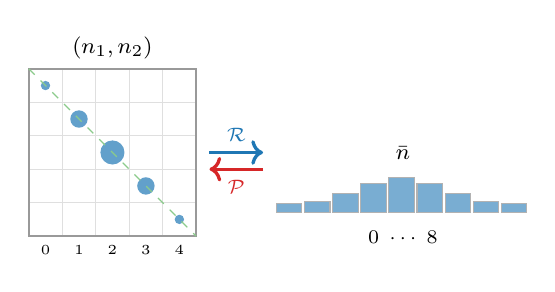
\begin{tikzpicture}[scale=0.85, every node/.style={font=\scriptsize}]
        % --- Fine grid ---
        \def\cs{0.50}
        \draw[gray!25](0,0) grid[step=\cs] (5*\cs,5*\cs);
        \draw[black!40,thick](0,0) rectangle (5*\cs,5*\cs);
        \node[above,font=\footnotesize] at (1.25,2.5) {$(n_1,n_2)$};
        % example mass
        \fill[coarsecolor!70](0.25,2.25) circle (0.07cm);
        \fill[coarsecolor!70](0.75,1.75) circle (0.13cm);
        \fill[coarsecolor!70](1.25,1.25) circle (0.18cm);
        \fill[coarsecolor!70](1.75,0.75) circle (0.13cm);
        \fill[coarsecolor!70](2.25,0.25) circle (0.07cm);
        \draw[coarsegreen!55,dashed](0,2.5)--(2.5,0);
        \foreach \n in {0,1,2,3,4}
          \node[below,font=\tiny] at ({(\n+0.5)*\cs},0) {\n};

        % Arrow
        \draw[->,very thick,coarsecolor] (2.7,1.25) -- (3.5,1.25)
          node[above,midway,font=\scriptsize]{$\calR$};
        \draw[->,very thick,slowred]     (3.5,1.0)  -- (2.7,1.0)
          node[below,midway,font=\scriptsize]{$\calP$};

        % --- Coarse bar ---
        \def\cb{0.42}
        \foreach \nb in {0,1,2,3,4,5,6,7,8} {
          \pgfmathsetmacro{\ht}{0.12 + 0.40*exp(-0.5*((\nb-4)/1.5)*((\nb-4)/1.5))}
          \fill[coarsecolor!60] (3.7+\nb*\cb, 0.35) rectangle
                                (3.7+\nb*\cb+\cb-0.04, 0.35+\ht);
          \draw[black!30] (3.7+\nb*\cb, 0.35) rectangle
                          (3.7+\nb*\cb+\cb-0.04, 0.35+\ht);
        }
        \node[above,font=\footnotesize] at (3.7+4*\cb+\cb/2, 1.0) {$\bar n$};
        \node[below,font=\scriptsize]   at (3.7+4.5*\cb, 0.22) {$0\;\cdots\;8$};
      \end{tikzpicture}

      \vspace{0.3em}
      {\footnotesize
        Summing along constant-total diagonals (left) gives
        the 1-D total $\bar n$ (right).
        Reconstruction spreads mass back via Binomial.
      }
      \end{center}
    \end{column}
  \end{columns}

\end{frame}


% ================================================================
%  3b.  What coarsening does to the generator
% ================================================================

\begin{frame}{What merging does to the rate matrix}

  \begin{columns}[T]
    \begin{column}{0.44\textwidth}
      \textbf{Full rate matrix $A$ — 4 voxels:}

      \begin{center}
      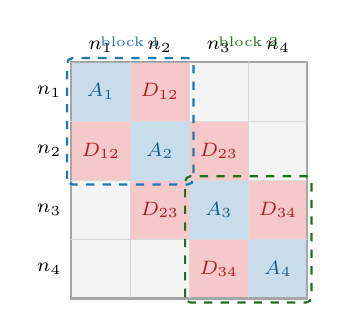
\begin{tikzpicture}[scale=0.75]
        \def\bs{1.00}
        \fill[gray!8] (0,0) rectangle (4*\bs,4*\bs);
        % Diagonal: reaction blocks A_k
        \foreach \k in {0,...,3}
          \fill[myblue!25] (\k*\bs,{(3-\k)*\bs}) rectangle ({(\k+1)*\bs},{(4-\k)*\bs});
        % Off-diagonal: diffusion D_{k,k+1}
        \foreach \k/\kp in {0/1,1/2,2/3} {
          \fill[slowred!25] (\kp*\bs,{(3-\k)*\bs}) rectangle ({(\kp+1)*\bs},{(4-\k)*\bs});
          \fill[slowred!25] (\k*\bs,{(3-\kp)*\bs}) rectangle ({(\k+1)*\bs},{(4-\kp)*\bs});
        }
        % Grid
        \draw[black!35,thick] (0,0) rectangle (4*\bs,4*\bs);
        \foreach \k in {1,...,3} {
          \draw[black!15,thin] (\k*\bs,0) -- (\k*\bs,4*\bs);
          \draw[black!15,thin] (0,\k*\bs) -- (4*\bs,\k*\bs);
        }
        % Labels
        \foreach \k/\l in {0/1,1/2,2/3,3/4}
          \node[font=\scriptsize,myblue!80!black]
            at ({(\k+0.5)*\bs},{(3.5-\k)*\bs}) {$A_\l$};
        \node[font=\scriptsize,slowred!80!black] at (1.5*\bs,3.5*\bs) {$D_{12}$};
        \node[font=\scriptsize,slowred!80!black] at (0.5*\bs,2.5*\bs) {$D_{12}$};
        \node[font=\scriptsize,slowred!80!black] at (2.5*\bs,2.5*\bs) {$D_{23}$};
        \node[font=\scriptsize,slowred!80!black] at (1.5*\bs,1.5*\bs) {$D_{23}$};
        \node[font=\scriptsize,slowred!80!black] at (3.5*\bs,1.5*\bs) {$D_{34}$};
        \node[font=\scriptsize,slowred!80!black] at (2.5*\bs,0.5*\bs) {$D_{34}$};
        % Axis
        \foreach \k/\l in {0/$n_1$,1/$n_2$,2/$n_3$,3/$n_4$} {
          \node[above,font=\scriptsize] at ({(\k+0.5)*\bs},4*\bs) {\l};
          \node[left, font=\scriptsize] at (0,{(3.5-\k)*\bs}) {\l};
        }
        % Pair brackets
        \draw[coarsecolor,thick,dashed,rounded corners=2pt]
          (-0.07,{2*\bs-0.07}) rectangle ({2*\bs+0.07},{4*\bs+0.07});
        \draw[coarsegreen!70!black,thick,dashed,rounded corners=2pt]
          ({2*\bs-0.07},{-0.07}) rectangle ({4*\bs+0.07},{2*\bs+0.07});
        \node[coarsecolor,font=\tiny,above] at (\bs,4*\bs+0.1) {block 1};
        \node[coarsegreen!70!black,font=\tiny,above] at (3*\bs,4*\bs+0.1) {block 2};
      \end{tikzpicture}
      \end{center}
      {\footnotesize Size: $n_{\max}^4$}
    \end{column}
    %
    \begin{column}{0.10\textwidth}
      \vspace{2.6cm}
      \begin{center}
        $\xrightarrow{\;\calR\;}$\\[0.5em]
        $\xleftarrow{\;\calP\;}$
      \end{center}
    \end{column}
    %
    \begin{column}{0.42\textwidth}
      \textbf{Merged rate matrix $\bar A$ — 2 blocks:}

      \begin{center}
      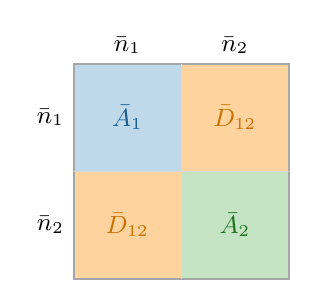
\begin{tikzpicture}[scale=0.75]
        \def\cs{1.82}
        \fill[gray!8] (0,0) rectangle (2*\cs,2*\cs);
        % Diagonal: coarsened reaction blocks
        \fill[coarsecolor!28]       (0,\cs) rectangle (\cs,2*\cs);
        \fill[coarsegreen!28]       (\cs,0) rectangle (2*\cs,\cs);
        % Off-diagonal: inter-group diffusion (boundary only)
        \fill[intercolor!38] (0,0) rectangle (\cs,\cs);
        \fill[intercolor!38] (\cs,\cs) rectangle (2*\cs,2*\cs);
        % Grid
        \draw[black!35,thick] (0,0) rectangle (2*\cs,2*\cs);
        \draw[black!15,thin] (\cs,0) -- (\cs,2*\cs);
        \draw[black!15,thin] (0,\cs) -- (2*\cs,\cs);
        % Labels
        \node[font=\small,coarsecolor!80!black]     at (0.5*\cs,1.5*\cs) {$\bar A_1$};
        \node[font=\small,coarsegreen!70!black]     at (1.5*\cs,0.5*\cs) {$\bar A_2$};
        \node[font=\small,intercolor!80!black]      at (0.5*\cs,0.5*\cs) {$\bar D_{12}$};
        \node[font=\small,intercolor!80!black]      at (1.5*\cs,1.5*\cs) {$\bar D_{12}$};
        % Axis
        \node[above,font=\small] at (0.5*\cs,2*\cs) {$\bar n_1$};
        \node[above,font=\small] at (1.5*\cs,2*\cs) {$\bar n_2$};
        \node[left, font=\small] at (0,1.5*\cs) {$\bar n_1$};
        \node[left, font=\small] at (0,0.5*\cs) {$\bar n_2$};
      \end{tikzpicture}
      \end{center}
      {\footnotesize Size: $n_{\max}^2$ \quad ($\mathbf{10^4\times}$ smaller for $n_{\max}{=}100$)}
      \begin{itemize}\setlength\itemsep{0.15em}
        \item \textcolor{myblue!80!black}{$A_k$} $\to$
              \textcolor{coarsecolor!80!black}{$\bar A_j$}:
              reactions averaged over the Binomial
        \item \textcolor{slowred!80!black}{Within-block $D$} disappears —
              implicit in the Binomial
        \item \textcolor{intercolor!80!black}{$\bar D_{12}$}: only
              between-block diffusion remains
      \end{itemize}
    \end{column}
  \end{columns}

\end{frame}

\begin{frame}{Merging fails at a bistable front}

  \begin{columns}[T]
    \begin{column}{0.38\textwidth}
      \textbf{Schl\"ogl model} ($K{=}8$, $S{=}1$):
      each voxel has two stable states.

      \medskip
      A \textbf{front} forms when neighboring voxels
      occupy opposite stable states.
      Slow diffusion ($d \ll$ reaction rates) sustains it indefinitely.

      \medskip
      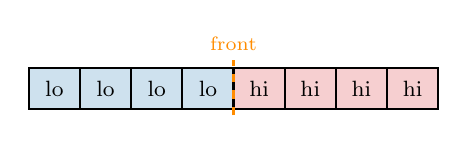
\begin{tikzpicture}[scale=0.65, every node/.style={font=\footnotesize}]
        \foreach \k in {1,2,3,4} {
          \draw[thick,fill=myblue!22] (\k-1,0) rectangle (\k,0.8);
          \node at (\k-0.5,0.4) {lo};
        }
        \foreach \k in {5,6,7,8} {
          \draw[thick,fill=slowred!22] (\k-1,0) rectangle (\k,0.8);
          \node at (\k-0.5,0.4) {hi};
        }
        \draw[very thick,intercolor,dashed] (4,-0.12) -- (4,0.96);
        \node[intercolor,above,font=\scriptsize] at (4,0.96) {front};
      \end{tikzpicture}

      \medskip
      At the front: the joint distribution of the two interface voxels is
      \emph{bimodal} — concentrated at $(n_{\rm lo},n_{\rm hi})$
      and $(n_{\rm hi},n_{\rm lo})$.\\[0.4em]
      The Binomial is \textbf{unimodal}: wrong shape.
    \end{column}
    \begin{column}{0.58\textwidth}
      \begin{center}
        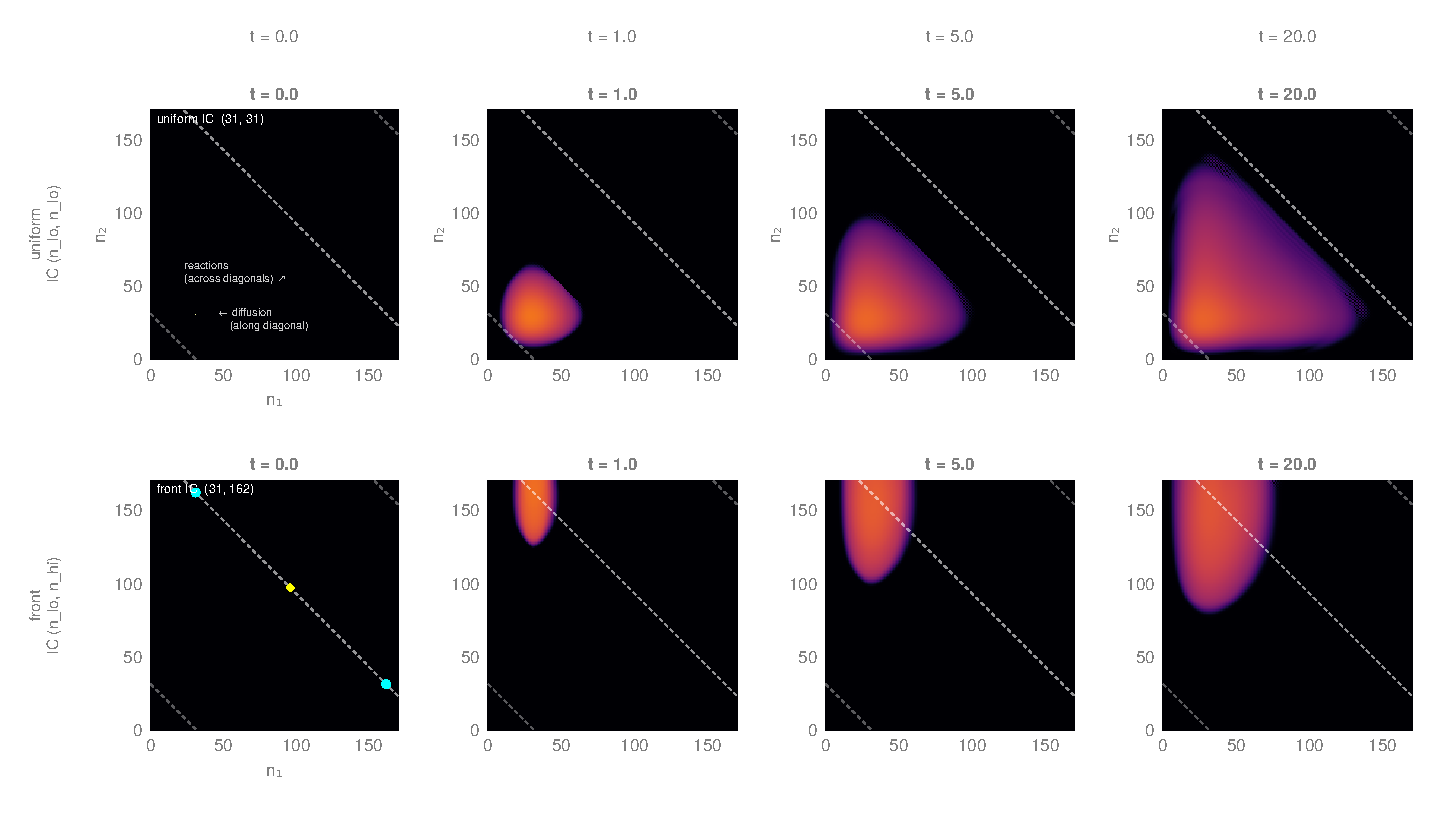
\includegraphics[width=\textwidth,keepaspectratio]{fig_prob_diffusion}
      \end{center}
      {\footnotesize
        \textbf{Top:} uniform initial condition — probability spreads along
        constant-total diagonals; Binomial reconstruction is accurate. \textcolor{coarsegreen!80!black}{\checkmark}\\
        \textbf{Bottom:} bistable front — probability stays at the corners;
        Binomial reconstruction gives the wrong shape. \textcolor{slowred}{\ding{55}}
      }
    \end{column}
  \end{columns}

\end{frame}


% ================================================================
%  5.  Detecting imbalance: the criterion
% ================================================================

\begin{frame}{When is merging valid? The imbalance criterion}

  \begin{columns}[T]
    \begin{column}{0.48\textwidth}
      Compare mean counts in adjacent voxels $2j{-}1$ and $2j$:
      \[
        \alpha_j = \frac{|\mu_{2j-1} - \mu_{2j}|}{\mu_{2j-1}+\mu_{2j}}.
      \]

      \begin{itemize}\setlength\itemsep{0.4em}
        \item Small $\alpha_j$: voxels balanced
              $\Rightarrow$ distribution near-Binomial $\Rightarrow$ safe to merge.
        \item Large $\alpha_j$: voxels in opposite states
              $\Rightarrow$ front is nearby $\Rightarrow$ keep fine.
      \end{itemize}

      \smallskip
      \begin{block}{Merging criterion}
        Find the most imbalanced block: $j^* = \operatorname{argmax}_j\,\alpha_j$.\\[0.2em]
        Keep $j^*$ and its immediate neighbors fine; merge all others.
      \end{block}
    \end{column}
    \begin{column}{0.48\textwidth}
      \begin{center}
        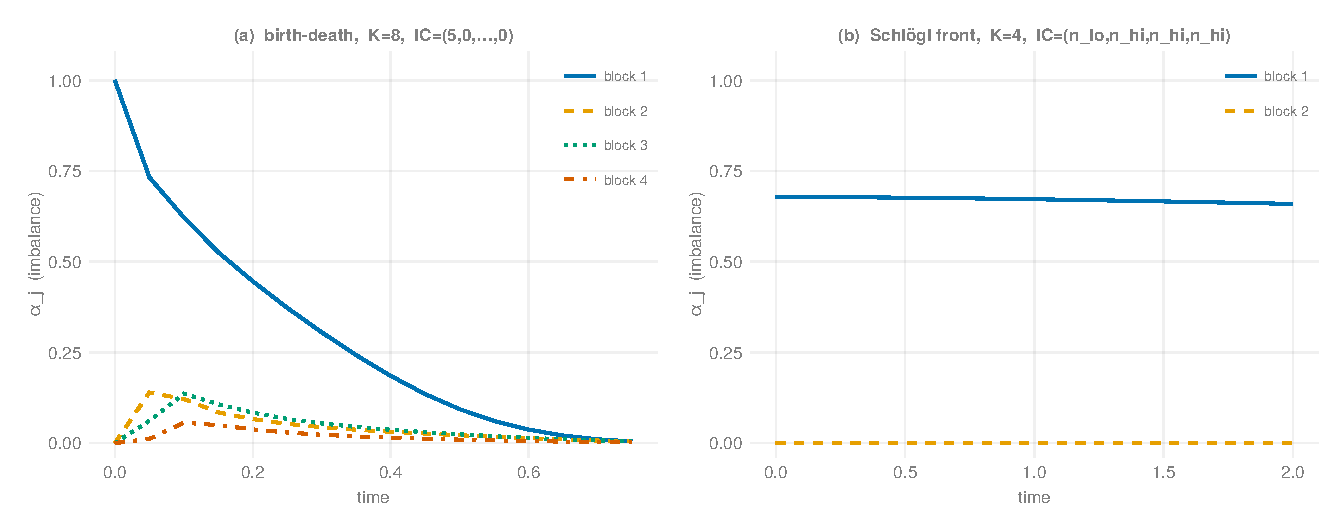
\includegraphics[width=\textwidth,keepaspectratio]{fig_criterion}
      \end{center}
      {\footnotesize
        \textbf{(a)} Birth-death: $\alpha_1$ decays to zero as diffusion equilibrates the two voxels.\\
        \textbf{(b)} Schl\"ogl front: $\alpha_1$ stays near 1 — the front is persistent.\\
        Green band = safe region for merging.
      }
    \end{column}
  \end{columns}

\end{frame}


% ================================================================
%  6.  The adaptive algorithm
% ================================================================

\begin{frame}{Adaptive algorithm: mixed-resolution evolution}

  \textbf{Idea.} Keep a fine window at the front; coarsen everything else.
  Evolve the mixed state \emph{directly} — no reconstruction step.

  \medskip
  \begin{columns}[T]
    \begin{column}{0.52\textwidth}
      \textbf{Mixed state $p^M$:}
      \begin{itemize}\setlength\itemsep{0.3em}
        \item \textcolor{coarsecolor}{\textbf{Coarse groups}}: only the total $\bar n_j$
              is tracked; split assumed Binomial.
        \item \textcolor{slowred}{\textbf{Fine group at front}}: both voxel counts
              $(n_{2j-1}, n_{2j})$ tracked exactly.
      \end{itemize}

      \medskip
      \textbf{Evolution:}
      $\dot p^M = A^M p^M$,
      where $A^M$ couples merged and fine blocks at block boundaries.

      \smallskip
      \textbf{Reassignment:} recompute $\alpha_j$ only when the front crosses a block boundary;
      update the fine window to be centered on $\operatorname{argmax}_j\,\alpha_j$.\\
      {\footnotesize\textit{Scope: one dominant, monotone-drifting front.}}
    \end{column}
    \begin{column}{0.44\textwidth}
      \begin{center}
      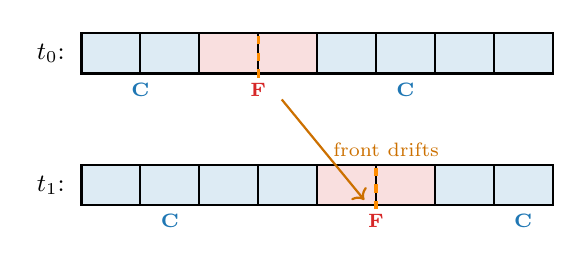
\begin{tikzpicture}[scale=0.88, every node/.style={font=\footnotesize}]
        \def\vh{0.58}
        \def\vw{0.85}

        % t0
        \node[left,font=\small] at (-0.1, 1.5*\vh) {$t_0$:};
        \foreach \k/\col in {1/coarsecolor!15,2/coarsecolor!15,3/slowred!15,4/slowred!15,5/coarsecolor!15,6/coarsecolor!15,7/coarsecolor!15,8/coarsecolor!15} {
          \draw[thick,fill=\col] ({(\k-1)*\vw},\vh) rectangle ({\k*\vw},{2*\vh});
        }
        \node[coarsecolor,font=\scriptsize\bfseries] at ({1*\vw},0.6*\vh) {C};
        \node[slowred,font=\scriptsize\bfseries]     at ({3*\vw},0.6*\vh) {F};
        \node[coarsecolor,font=\scriptsize\bfseries] at ({5.5*\vw},0.6*\vh) {C};
        \draw[very thick,intercolor,dashed] ({3*\vw},0.9*\vh) -- ({3*\vw},2.1*\vh);

        % t1
        \node[left,font=\small] at (-0.1, 1.5*\vh - 1.9) {$t_1$:};
        \foreach \k/\col in {1/coarsecolor!15,2/coarsecolor!15,3/coarsecolor!15,4/coarsecolor!15,5/slowred!15,6/slowred!15,7/coarsecolor!15,8/coarsecolor!15} {
          \draw[thick,fill=\col] ({(\k-1)*\vw},\vh-1.9) rectangle ({\k*\vw},{2*\vh-1.9});
        }
        \node[coarsecolor,font=\scriptsize\bfseries] at ({1.5*\vw},0.6*\vh-1.9) {C};
        \node[slowred,font=\scriptsize\bfseries]     at ({5*\vw},0.6*\vh-1.9)   {F};
        \node[coarsecolor,font=\scriptsize\bfseries] at ({7.5*\vw},0.6*\vh-1.9) {C};
        \draw[very thick,intercolor,dashed] ({5*\vw},0.9*\vh-1.9) -- ({5*\vw},2.1*\vh-1.9);

        % Drift arrow
        \draw[->,thick,intercolor!80!black] ({3.4*\vw},0.7*\vh-0.2) -- ({4.8*\vw},0.7*\vh-1.65)
          node[midway,right,font=\scriptsize]{front drifts};
      \end{tikzpicture}
      \end{center}
      {\footnotesize
        Fine window follows the front.
        Coarse regions stay compressed.
      }
    \end{column}
  \end{columns}

\end{frame}


% ================================================================
%  6b.  Algorithm
% ================================================================

\begin{frame}{One time step of the adaptive solver}

  \textbf{Every step:}
  \begin{enumerate}\setlength\itemsep{0.25em}
    \item \textbf{Solve:} $p^M \leftarrow e^{\Delta t\, A^M}\, p^M$
    \item \textbf{Truncate/expand:} drop states below threshold $\tau$;
          add one-step reachable states (adaptive FSP)
    \item \textbf{Track front:} compute weighted mean block position $\bar\jmath$
          from voxel means — $O(|\mathcal{S}^M|)$, cheap
  \end{enumerate}

  \medskip
  \textbf{Only when front crosses a block boundary} ($|\bar\jmath - \bar\jmath_{\rm prev}| \geq \tfrac{1}{2}$):
  \begin{enumerate}\setlength\itemsep{0.25em}\setcounter{enumi}{3}
    \item \textbf{Re-evaluate} $\alpha_j$ for all blocks; find $j^* = \operatorname{argmax}_j\,\alpha_j$
    \item \textbf{Update partition:}
          keep $j^*$ and its neighbors fine; merge all other blocks
    \item \textbf{Transfer state:}
          split blocks $\to$ fine via $\Bin(\bar n_j,\tfrac12)$;\;
          merged blocks $\to$ compressed via $\bar n_j = n_{2j-1}+n_{2j}$
  \end{enumerate}

\end{frame}



\begin{frame}{Results: adaptive criterion eliminates merging error}

  \begin{center}
    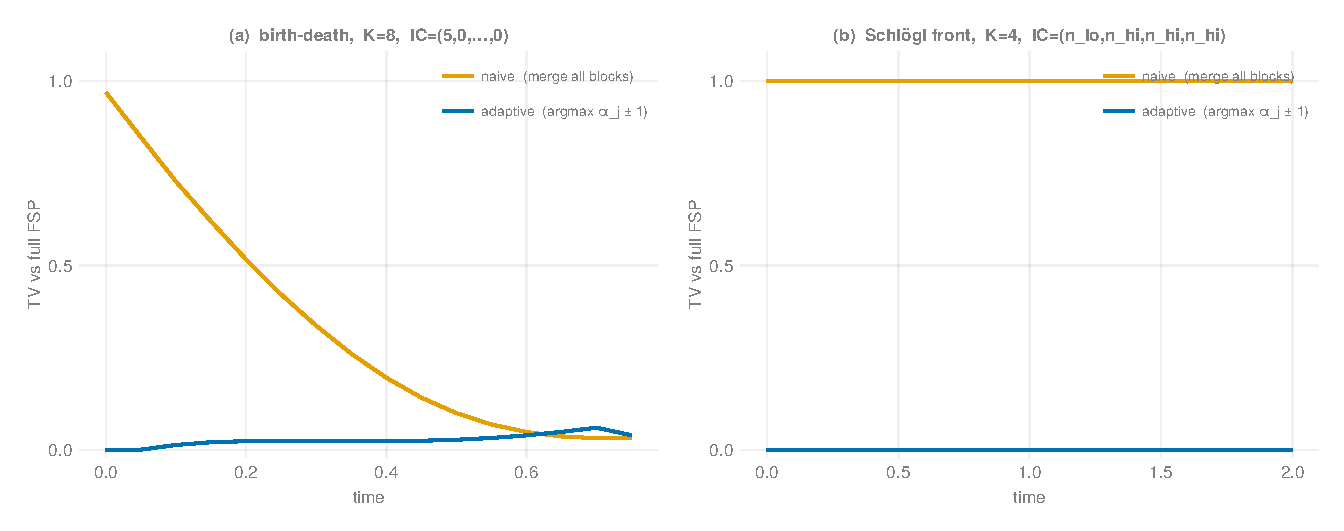
\includegraphics[width=0.88\textwidth,keepaspectratio]{fig_tv_criterion}
  \end{center}

  {\footnotesize
    Total variation distance from the reference (full FSP).\\
    \textbf{(a)} Birth-death: merging from $t{=}0$ gives large transient TV.
    Adaptive (merge only away from $\operatorname{argmax}_j\,\alpha_j$): TV $\to 0$ after equilibration.\\
    \textbf{(b)} Schl\"ogl front: na\"ive merging gives TV $\approx 1$ throughout
    (interface orientation lost).
    Adaptive: TV $\approx 0$ throughout.
  }

\end{frame}


\begin{frame}{Results: adaptive mixed-resolution is accurate and fast}

  \begin{columns}[T]
    \begin{column}{0.50\textwidth}
      \begin{center}
        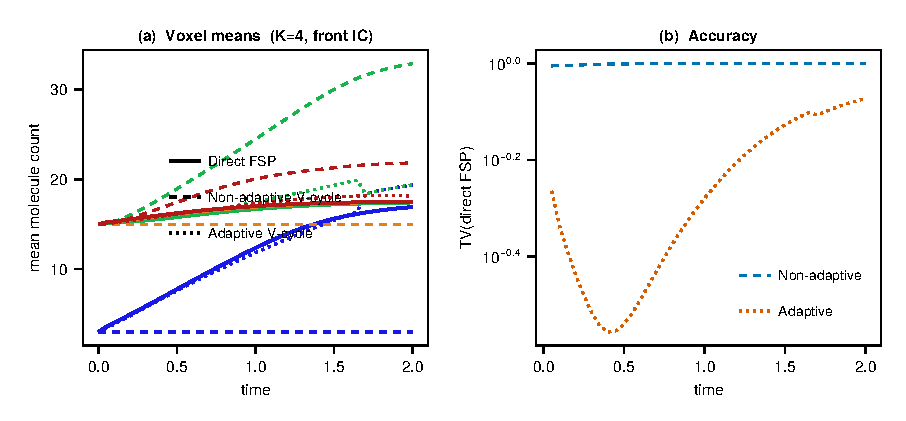
\includegraphics[width=\textwidth,keepaspectratio]{fig_adaptive_accuracy}
      \end{center}
      {\footnotesize Voxel means: adaptive mixed-resolution vs.\ full FSP.
      Means match; TV error is small but nonzero (see left panel).}
    \end{column}
    \begin{column}{0.46\textwidth}
      \begin{center}
        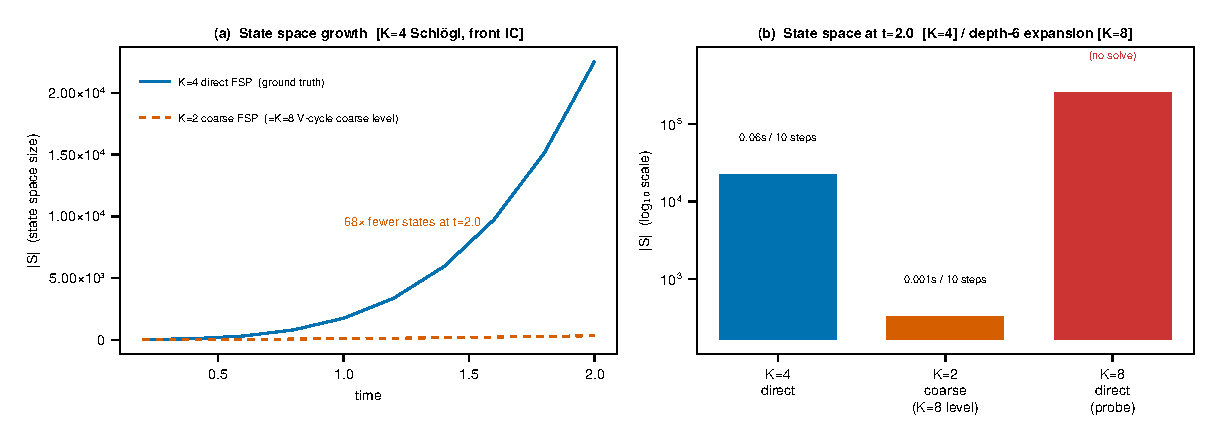
\includegraphics[width=\textwidth,keepaspectratio]{fig_speedup}
      \end{center}
      {\footnotesize
        State-space size across $K$.
        Mixed-resolution is dramatically smaller;
        full FSP at large $K$ is infeasible.
        \textit{(Size comparison, not a timing benchmark.)}
      }
    \end{column}
  \end{columns}

\end{frame}


% ================================================================
%  8.  Summary
% ================================================================

\begin{frame}{Summary}

  \begin{block}{1.\quad Fast diffusion enables state-space compression.}
    When the joint distribution of two adjacent voxels is near $\Bin(\bar n,\tfrac12)$
    (verified at runtime via $\alpha_j$),
    Replacing $(n_1,n_2)$ by $\bar n$ cuts the per-group state space
    from $n_{\max}^{2S}$ to $n_{\max}^{S}$.
  \end{block}

  \smallskip
  \begin{block}{2.\quad Bistable fronts violate the Binomial assumption.}
    Reactions keep neighboring voxels in opposite stable states,
    producing a bimodal conditional — not Binomial.
    The imbalance $\alpha_j$ detects this automatically.
  \end{block}

  \smallskip
  \begin{block}{3.\quad Adaptive mixed-resolution FSP.}
    Maintain a fine window at the front; coarsen the rest.
    Evolve $\dot p^M = A^M p^M$ directly — no reconstruction step.
    \textbf{Accurate and tractable for $K$ where full FSP is not.}
  \end{block}

  \smallskip
  \textbf{Scope \& open questions.}
  Current: 1D, single dominant interface, empirical criterion.
  Open: rigorous error bound; multi-species; multiple fronts.

\end{frame}


% ================================================================
\appendix
% ================================================================

\begin{frame}{Appendix: why not reconstruct after every step?}

  \textbf{Na\"ive approach:} pre-equilibrate $\to$ compress $\to$ coarse solve $\to$ reconstruct.

  \medskip
  \begin{columns}[T]
    \begin{column}{0.50\textwidth}
      \begin{center}
      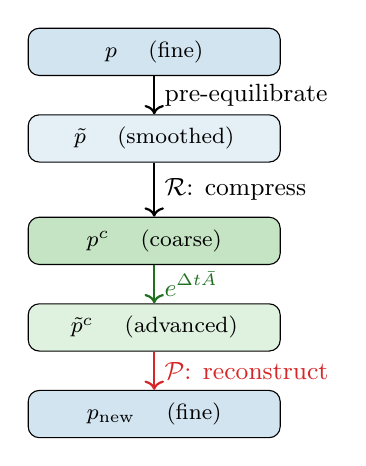
\begin{tikzpicture}[every node/.style={font=\footnotesize},scale=1.0]
        \node[draw,rounded corners,fill=myblue!20,
              minimum width=3.2cm,minimum height=0.6cm]
          (f1) at (0,4.6) {$p$ \quad (fine)};
        \node[draw,rounded corners,fill=myblue!12,
              minimum width=3.2cm,minimum height=0.6cm]
          (f2) at (0,3.5) {$\tilde p$ \quad (smoothed)};
        \node[draw,rounded corners,fill=coarsegreen!28,
              minimum width=3.2cm,minimum height=0.6cm]
          (c1) at (0,2.2) {$p^c$ \quad (coarse)};
        \node[draw,rounded corners,fill=coarsegreen!15,
              minimum width=3.2cm,minimum height=0.6cm]
          (c2) at (0,1.1) {$\tilde p^c$ \quad (advanced)};
        \node[draw,rounded corners,fill=myblue!20,
              minimum width=3.2cm,minimum height=0.6cm]
          (f3) at (0,0.0) {$p_{\rm new}$ \quad (fine)};
        \draw[->,thick] (f1.south)--(f2.north) node[midway,right]{\small pre-equilibrate};
        \draw[->,thick] (f2.south)--(c1.north) node[midway,right]{\small $\calR$: compress};
        \draw[->,thick,coarsegreen!70!black] (c1.south)--(c2.north) node[midway,right]{\small $e^{\Delta t \bar A}$};
        \draw[->,thick,slowred] (c2.south)--(f3.north) node[midway,right]{\small $\calP$: reconstruct};
      \end{tikzpicture}
      \end{center}
    \end{column}
    \begin{column}{0.46\textwidth}
      \begin{alertblock}{Reconstruction is wrong at the front}
        Step 4 forces a Binomial split on \emph{every} group of adjacent voxels,
        including the front where the true distribution is bimodal.\\[0.5em]
        \textbf{Fix:} evolve $p^M$ directly — no reconstruction step.
        Coarse groups carry the Binomial assumption implicitly in $\bar A_j$;
        the fine group tracks the true within-group distribution exactly.
      \end{alertblock}
    \end{column}
  \end{columns}

\end{frame}


\begin{frame}{Appendix: mixed-resolution generator is self-consistent}

  \begin{center}
    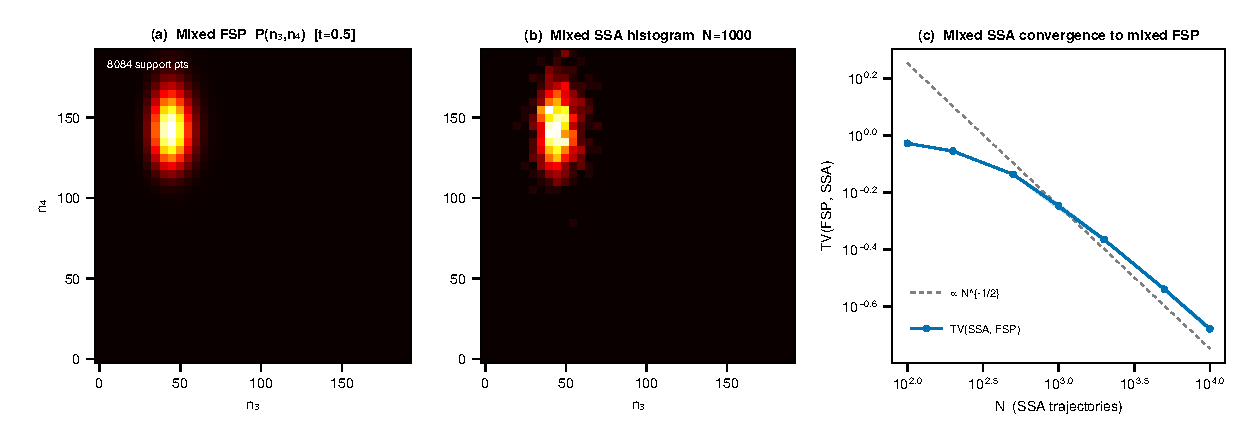
\includegraphics[width=0.78\textwidth,keepaspectratio]{fig_mixed_fsp_ssa}
  \end{center}

  {\footnotesize
    ODE solve on the mixed state $(\bar n_1, n_3, n_4)$
    vs.\ Monte Carlo on the \emph{same} reduced generator.
    Means agree to ${<}1\%$; TV $\sim N^{-1/2}$ (pure sampling noise).
    This confirms the solver is correct for the reduced model —
    not that the reduced model is unbiased relative to the full RDME.
  }

\end{frame}


\begin{frame}{Appendix: resolving interface orientation ($K{=}8$)}

  \begin{center}
    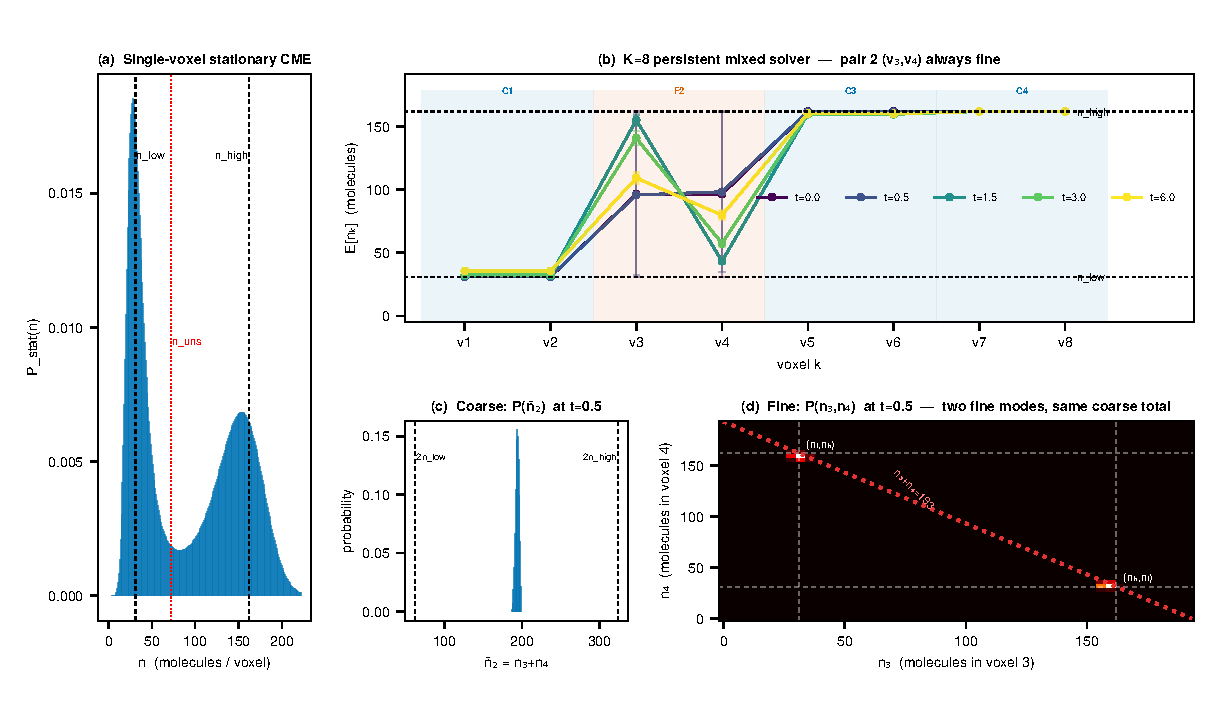
\includegraphics[width=0.78\textwidth,height=0.68\textheight,keepaspectratio]{fig_k8_persistent}
  \end{center}

  {\footnotesize
    IC: interface voxels in equal superposition of $(n_{\rm lo},n_{\rm hi})$ and $(n_{\rm hi},n_{\rm lo})$.
    \textbf{Coarse} $P(\bar n_2)$: single peak — orientation lost.
    \textbf{Fine} $P(n_3,n_4)$: two modes — mixed state retains the within-group structure.
  }

\end{frame}


\begin{frame}[allowframebreaks]{References}
  \footnotesize
  \begin{itemize}
    \item Erban, Chapman, Maini (2007). Stochastic simulations of reaction-diffusion.
      \textit{arXiv:0704.1908}.
    \item Munsky \& Khammash (2006). Finite State Projection.
      \textit{J.\ Chem.\ Phys.}, 124:044104.
    \item Briggs, Henson, McCormick (2000). \textit{A Multigrid Tutorial}, 2nd ed.\ SIAM.
    \item Dendukuri, Chandrasekaran, Petzold (2025).
      Adaptive multigrid FSP for the RDME. \textit{In preparation}.
  \end{itemize}
\end{frame}

\end{document}
